\newpage
\changeindent{0cm}
\section{要素技術}
\label{sec:tech}
\changeindent{2cm}

%9-12
本章では,本研究の提案手法に用いた技術について説明する.

%LSTM
\changeindent{0cm}
\subsection{深層学習}
\changeindent{2cm}
\label{sec:02_deep}



\changeindent{0cm}
\subsection{Neural Architecture Search}
\changeindent{2cm}
\label{sec:02_nas}
Neural Architecture Search(NAS)\cite{DBLP:journals/corr/ZophL16}は,
機械学習の分野で使用されているニューラルネットワークの設計を自動化する手法である.
ニューラルネットワークの設計は直感的でなく,
チューニングに人による労力を多く必要とするため,
ニューラルネットワークの設計は非常に困難である.

NASはニューラルネットワークが構造に関する設定の文字列で表現できることを利用して,
この文字列を生成する
Recurrent Neural Network(RNN)を
強化学習 Reinforcement Learning(RL)によって学習する.



\changeindent{0cm}
\subsection{Differentiable Architecture Search}
\changeindent{2cm}
\label{sec:02_darts}

Differentiable Architecture Search(DARTS)\cite{DBLP:journals/corr/abs-1806-09055}は,
離散的なアーキテクチャ探索空間に強化学習を適用したNASとは異なり,
微分可能な方法で定式化し,
偏微分による勾配降下法を使用してアーキテクチャを効率的に探索する手法である.

探索空間を連続にするため, カテゴリカルな演算子の選択の代わりに, 候補全ての可能性をもつ混合演算子を
(\ref{eq:darts/operation}) 式で定義する.
アーキテクチャを有向非巡回グラフで表したとき, ノードを潜在的な特徴表現 $x^{(i)}$,
エッジを特徴 $x^{(i)}$ が適用される関数 $o(・)$ とすると,
\begin{equation}
  \label{eq:darts/operation}
  \bar{o}^{(i, j)}(x) = \sum_{o \in \mathcal{O}} \frac{\exp(\alpha^{(i, j)}_o)}{\sum_{o' \in \mathcal{O}} \exp(\alpha^{(i, j)}_{o'})} o(x)
\end{equation}
となる. ここで
$\mathcal{O}$ は探索する演算子の候補集合,
$\alpha^{(i, j)}$ はエッジ $(i, j)$ の混合演算子の重みベクトルである.
DARTSは勾配降下法によって連続変数集合$\alpha$を学習する.

$\alpha$ とレイヤーの重み $w$ のBi-Level最適化問題を $w$ の近似によって同時に学習し,
NASにおいて 3000 GPU days 必要なタスクに対してDARTSは 3.3 GPU days まで高速化した.

DARTSでは次元を統一するためセルと呼ぶ小さなネットワーク構造を重ねたモデルを利用する.
セルを構成するノードは2つのノードからの演算子エッジを持ち,
どのノードからの演算子を選ぶのかをアーキテクチャを示す重み $\alpha$ によって決定する.
DARTSの問題点として位置と演算子の種類は探索できるが,
大局的な構造やノードの持つエッジ数など固定されたアーキテクチャにしか適用できない点が挙げられる.


\changeindent{0cm}
\subsection{Genetic Algorithm}
\changeindent{2cm}
\label{sec:02_ga}
遺伝的アルゴリズム(Genetic Algorithm : GA)は生物の進化の仕組みを模倣した最適化手法である.
問題の解候補を遺伝子の持つ個体として表現し, 適応度によって個体を評価・選択する.
交叉・突然変異などの操作によって解候補の多様性を保ちつつ,
近傍を探索しながら世代を重ねて近似的な最適解を求める.
% GAに必要な条件は評価関数の全順序性と探索空間が位相を持つことである.

% 整数値と実数値

% 初期収束問題
GAには偶然適応度の高くなった個体だけが選択され続け,
個体群を同じ個体が占める初期収束問題がある.
問題によって適切な交叉・突然変異を設定する必要がある.


\changeindent{0cm}
\subsection{Thermo?? Dinamic?? Genetic Algorithm}
\changeindent{2cm}
\label{sec:02_tdga}


% \begin{eqnarray}
% s_{t} &=& f(U_{x_{t}}+W_{s_{t-1}}) \nonumber \\
% y_{t} &=& g(V_{s_{t}}) \nonumber \\[8pt]
% f(z) &=& \frac{1}{1+\exp(-z)} \nonumber \\[8pt]
% g(z_{m}) &=& \frac{\exp(z_{m})}{\sum_{k}\exp(z_{k})} \nonumber
% \end{eqnarray}
%
% \begin{figure}[t]
%      \begin{center}
%        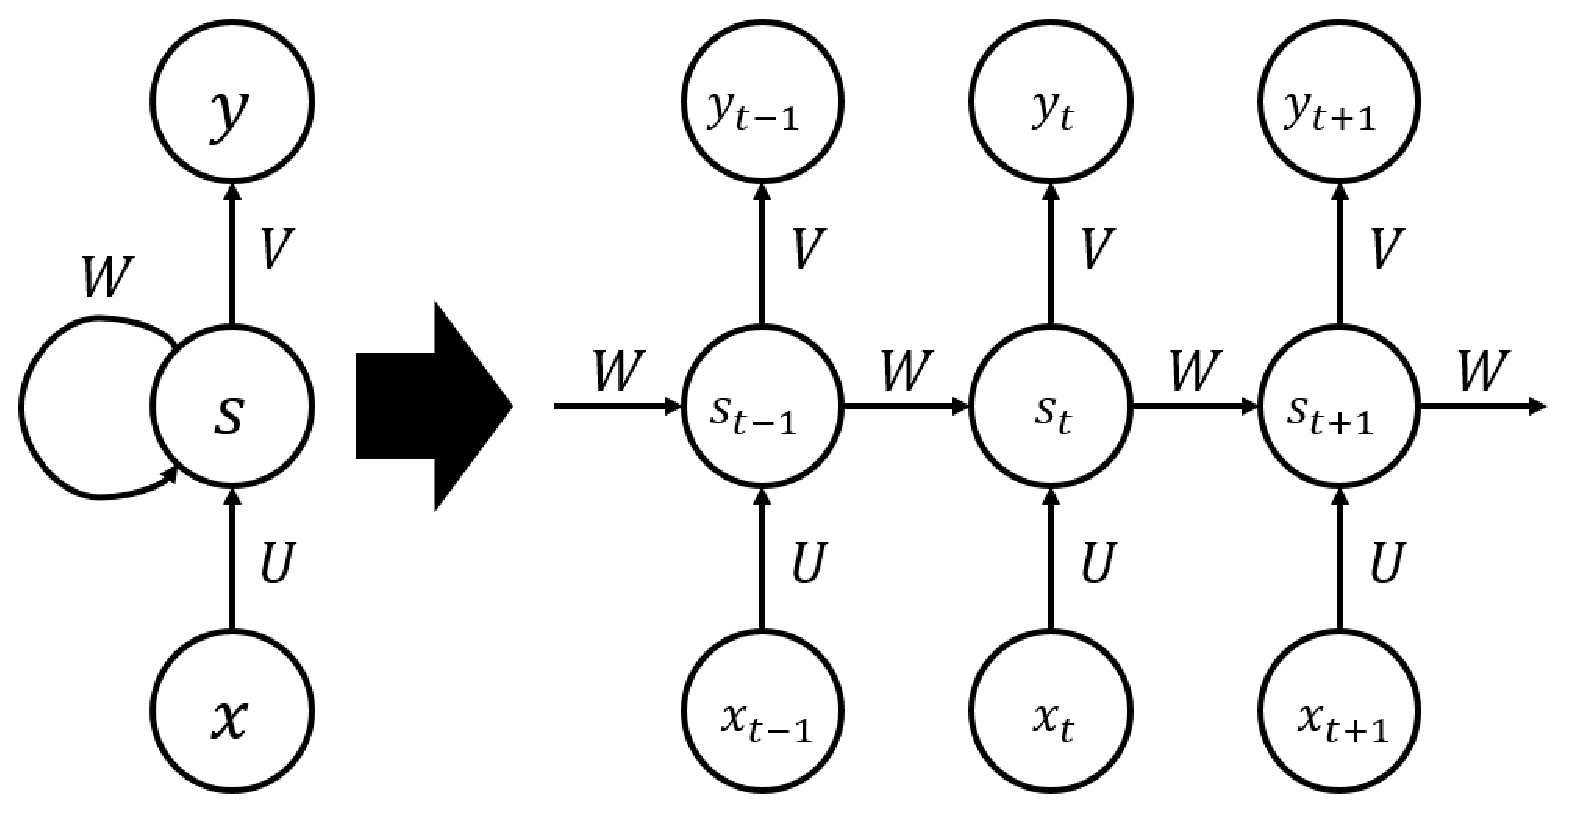
\includegraphics[width=12cm,clip]{./fig/02.tech/rnn.eps}
%       \end{center}
%       \caption{RNN ネットワーク}
%      \label{fig:02_net}
% \end{figure}
